\documentclass[a4paper,12pt]{article}
\usepackage{amsmath}
\usepackage{amssymb}
\usepackage[polish]{babel}
\usepackage{polski}
\usepackage[utf8]{inputenc}
\usepackage{indentfirst}
\usepackage{geometry}
\usepackage{array}
\usepackage[pdftex]{color,graphicx}
\usepackage{subfigure}
\usepackage{afterpage}
\usepackage{setspace}
\usepackage{color}
\usepackage{wrapfig}
\usepackage{listings}
\usepackage{datetime}

\renewcommand{\onehalfspacing}{\setstretch{1.6}}

\geometry{tmargin=2.5cm,bmargin=2.5cm,lmargin=2.5cm,rmargin=2.5cm}
\setlength{\parindent}{1cm}
\setlength{\parskip}{0mm}

\newenvironment{lista}{
\begin{itemize}
  \setlength{\itemsep}{1pt}
  \setlength{\parskip}{0pt}
  \setlength{\parsep}{0pt}
}{\end{itemize}}

\newcommand{\linia}{\rule{\linewidth}{0.4mm}}

\definecolor{lbcolor}{rgb}{0.95,0.95,0.95}
\lstset{
    backgroundcolor=\color{lbcolor},
    tabsize=4,
  language=C++,
  captionpos=b,
  tabsize=3,
  frame=lines,
  numbers=left,
  numberstyle=\tiny,
  numbersep=5pt,
  breaklines=true,
  showstringspaces=false,
  basicstyle=\footnotesize,
  identifierstyle=\color{magenta},
  keywordstyle=\color[rgb]{0,0,1},
  commentstyle=\color[rgb]{0,0.5,0},
  stringstyle=\color{red}
  }

\begin{document}

\noindent
\begin{tabular}{|c|p{11cm}|c|} \hline
Grupa 4 & Katarzyna Kosiak, Michał Folwarski & \ddmmyyyydate\today \tabularnewline
\hline 
\end{tabular}


\section*{Zadanie 4 - Liczby pierwsze -- OMP}
Program ma za zadanie wykonać test pierwszości (sprawdzić czy dana liczba jest liczbą pierwszą) na zestawie liczb zapisanym w~pliku.
Algorytm sprawdzania testu pierwszości został zaimplementowany na bazie metody naiwnej oraz optymalizacji~o:
\begin{lista}
 \item pominięcie liczb parzystych,
 \item pominięcie liczb podzielnych przez trzy,
 \item sprawdzenie dzielników tylko do pierwiastka kwadratowego sprawdzanej liczby.
\end{lista}

\begin{lstlisting}
#pragma omp parallel for num_threads(numberOfThreds) \
    default(none) shared(numbers) private(i) schedule(dynamic, 1)
for (i=0; i < numbers.size(); ++i) {
    // sprawdzenie czy dana liczba numbers[i] jest liczba pierwsza
}
\end{lstlisting}
Powyższy fragment kodu przedstawia w~jaki sposób zostało zorganizowane rozdzielanie zadań pomiędzy wątki w~OpenMP. W~tym zadaniu równomierne rozdzielenie zadań pomiędzy dostępne wątki nie sprawdzi się, ponieważ sprawdzenie czy podana liczba jest pierwszą będzie wykonywało się w~różnym czasie. Dzięki dyrektywie \verb!schedule! możemy kontrolować sposób rozdzielania iteracji. W~tym przypadku jest to rozdzielone dynamicznie na jednoelementowe podzbiory -- każdy z~wątków otrzyma jedną liczbę do sprawdzenia. Dzięki takiemu podziałowi, wątek otrzyma następne zadanie dopiero po zakończeniu poprzedniego. Zwiększanie ilości elementów w~podzbiorach powoduje, że otrzymane wyniki są nieznacznie większe lub mniejsze w~zależności od zestawu danych.

\begin{figure}[!hbp]
  \centering
    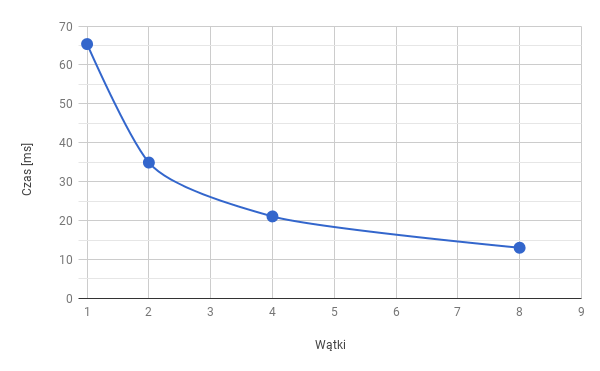
\includegraphics[width=0.7\textwidth]{chart}
  \caption{Wykres zależności czasu wykonania od ilości wątków}
  \label{chart-time-threads}
\end{figure}

Powyższy wykres przedstawia wyniki czasu obliczeń dla zestawu liczb znajdującym się na serwerze w~pliku \texttt{/home/shared/prir/primes/4.txt} -- odpowiednio dla jednego, dwóch, czterech i~ośmiu wątków. Zgodnie z~oczekiwaniami, czas obliczeń maleje wraz ze zwiększaniem liczby wątków do wykonywania obliczeń.

Na rysunku numer \ref{chart-acceleration} został przedstawiony wykres przyspieszenia obliczeń dla tego zestawu danych. Z~wykresu można odczytać, że wzrost szybkości obliczeń na ośmiu wątkach w~stosunku do obliczeń sekwencyjnych jest około pięciokrotny -- jest to spowodowane tym, iż do zarządzania wątkami oraz~przydziału im zadań, potrzebna jest pewna ilości zasobów (w tym także obliczeniowe).

\begin{figure}[!htbp]
  \centering
    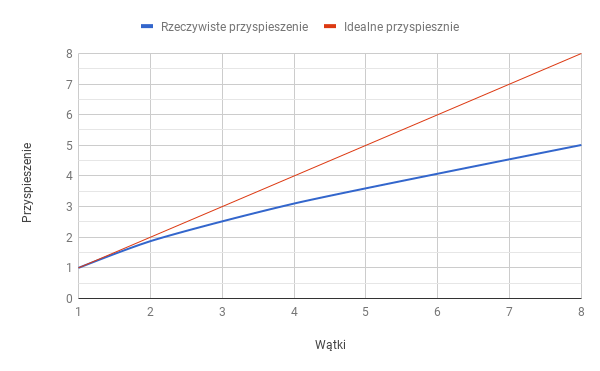
\includegraphics[width=0.7\textwidth]{chart2}
    \caption{Krzywa przyspieszenia obliczeń w~zależności od ilości wątków.}
  \label{chart-acceleration}
\end{figure}

\subsubsection*{Wnioski}
Dzięki zastosowaniu OpenMP, możliwe jest budowanie aplikacji do obliczeń równoległych jest proste -- wystarczy dodać kilka dyrektyw, aby otrzymać zadowalające wyniki. W~tym zadaniu przetestowaliśmy możliwość dynamicznego rozdzielenia zadań pomiędzy wątki, a~co w~naszym przypadku przyniosło oczekiwane rezultaty -- obliczenia zostały zrównoleglone pomiędzy wątki i~dzięki temu zwiększyła się szybkość obliczeń.

\end{document}
